%!TEX TS-program = xelatex
%!TEX encoding = UTF-8 Unicode

\documentclass[11pt,tikz,border=1]{standalone}

\begin{document}
  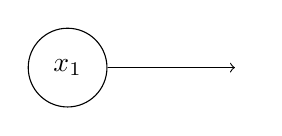
\begin{tikzpicture}[
    neuron/.style={circle,draw,inner sep=0pt,minimum size=10mm}
    ]

    \node (perceptron) at (0, 0) [neuron] {$x_1$};
    \node (output) at (2.25, 0) {};
    \draw [->] (perceptron) to (output);

  \end{tikzpicture} 
\end{document}
